\section{Experimental Evaluation}\label{sec:exp}

\subsection{Experiment Settings}

We evaluate the proposed technique over the FourSquare check-in dataset~\cite{yang2014modeling}. The dataset contains 227,428 check-ins in New York city and 573,703 check-ins in Tokyo collected in 10 month. A PoI type is given for each record. We use the user ratings on FourSquare as ground truth. Specifically, FourSquare uses a 10-point rating system, but a user cannot give arbitrary points to a PoI. A user can select from three options: ``Like" (count as 10 points), ``Neither like nor dislike" (count as 5 points), or ``Dislike" (count as 0 point). Which PoI is liked by a user is publicly available. We have implemented three schemes:
\begin{itemize}
\item{Linear regression (LR)} A baseline approach that predicts user ratings with a model generated by simple linear regression with the proposed features.
\item{Matrix factorization (MF)} The simple non-negative matrix factorization~\cite{koren2009matrix} for recommender systems. We use matrix factorization to predict the rating of each users who have visited a PoI, and then use their average rating score as the ``overall" rating of the PoI.
\item{Deep neural network (DNN)} The scheme predicts user ratings with a model trained by deep neural network as proposed in Section~\ref{sec:prediction}, using the proposed features.
\end{itemize}

For LR and DNN, we use the four types of features discussed in Section~\ref{sec:method}. More parameters of our experiment is given in Table~\ref{settings}. Our experiment platform is a virtual machine with Intel Xeon 64-bit 8-core CPU running on 2.93GHz and 32GB RAM. The algorithms are implemented with Microsoft Azure machine learning toolkit and modules. 

\begin{table}[htbp]
\begin{center}
\caption{Groups based on how often user visits a location \label{settings}}
\begin{tabular}{|l|l|} \hline
\textbf{Parameter} & \textbf{Default value} \\ \hline
Number of users & 5000  \\ \hline
Number of PoIs & 1500 \\ \hline
Training set size (\%) & 10\% \\ \hline
Cost function & Mean Square Error \\ \hline
Neural network depth (for DNN)& 4 \\ \hline
Neurons per layer (for DNN) & 12 \\ \hline
Output function (for DNN) & sigmoid \\ \hline
Number of latent features (for MF) & 8 \\ \hline
\end{tabular}
\end{center}
\end{table}

\subsection{Data Cleaning}

A few data cleaning steps are needed to prepare the dataset. First, we remove the \textit{inactive} users from the dataset. We define inactive users as those who have less than 1 check-ins per week in the 10 month period, and have less than 10 liked locations. The lack of data makes it hard to extra features for these users. Second, we remove the PoIs which were not rated by any of these users, since the ground truth is not available for such PoI. After the cleaning process, we extract the check-in information of approximately 5000 most active users and 1500 PoIs they have visited from the dataset.

In order for MF to work, we also generate a user-PoI rating matrix based on the users and PoIs appeared in the FourSquare dataset. The user ratings are directly crawled from FourSquare.


\subsection{Prediction Results}

\begin{figure}[ht]%
        \centering
        \begin{subfigure}{0.25\textwidth}
               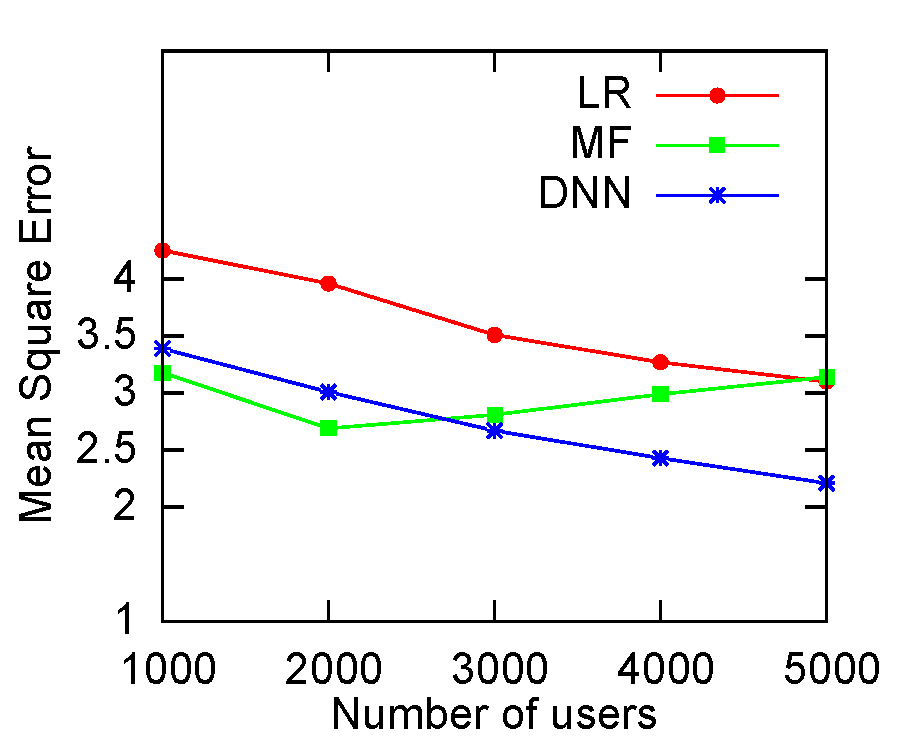
\includegraphics[scale=0.25]{E1.pdf}
        \end{subfigure}%
        ~ %add desired spacing between images, e. g. ~, \quad, \qquad, \hfill etc.
          %(or a blank line to force the subfigure onto a new line)
        \begin{subfigure}{0.25\textwidth}
                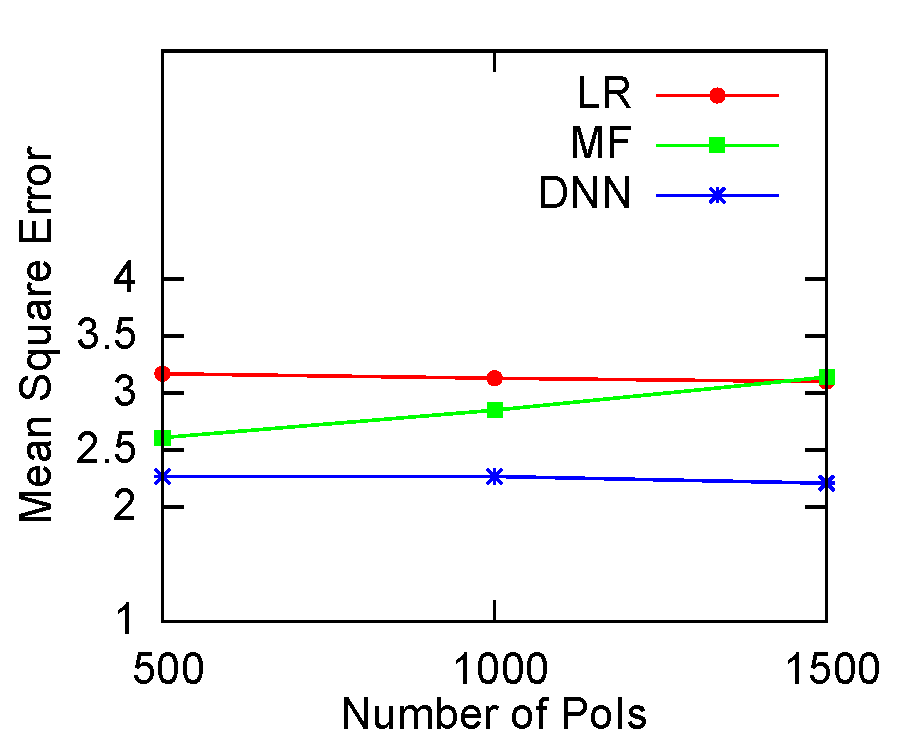
\includegraphics[scale=0.25]{E2.pdf}
        \end{subfigure}
         \caption{MSE of different prediction schemes}\label{E12}
         \vspace{-2mm}
\end{figure}

\begin{figure}[htb]%
        \centering
        \begin{subfigure}{0.25\textwidth}
               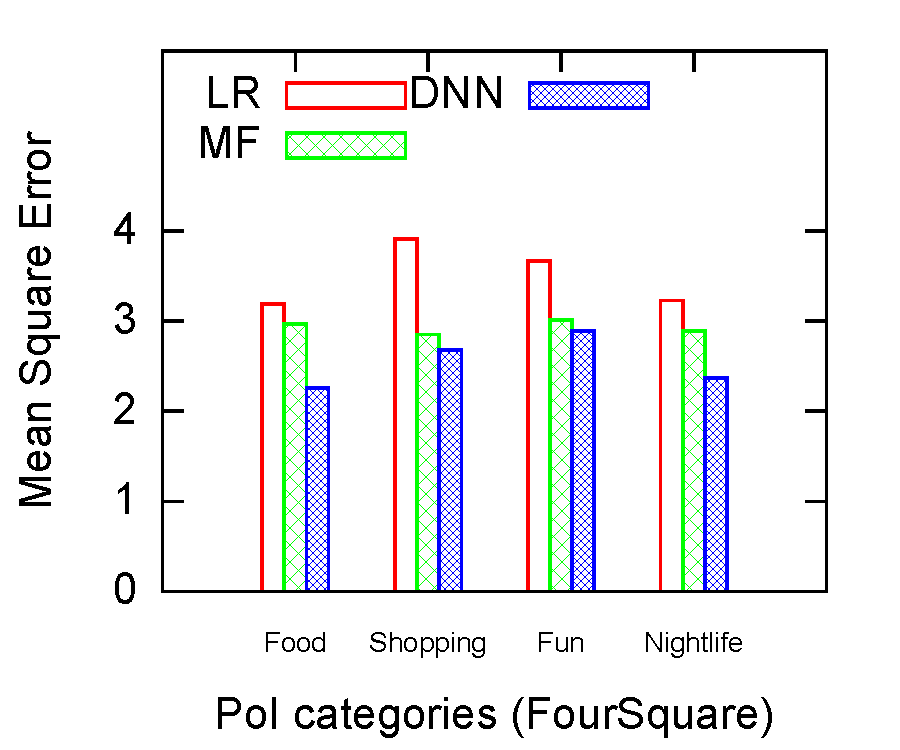
\includegraphics[scale=0.25]{E3-a.pdf}
        \end{subfigure}%
        ~ %add desired spacing between images, e. g. ~, \quad, \qquad, \hfill etc.
          %(or a blank line to force the subfigure onto a new line)
        \begin{subfigure}{0.25\textwidth}
                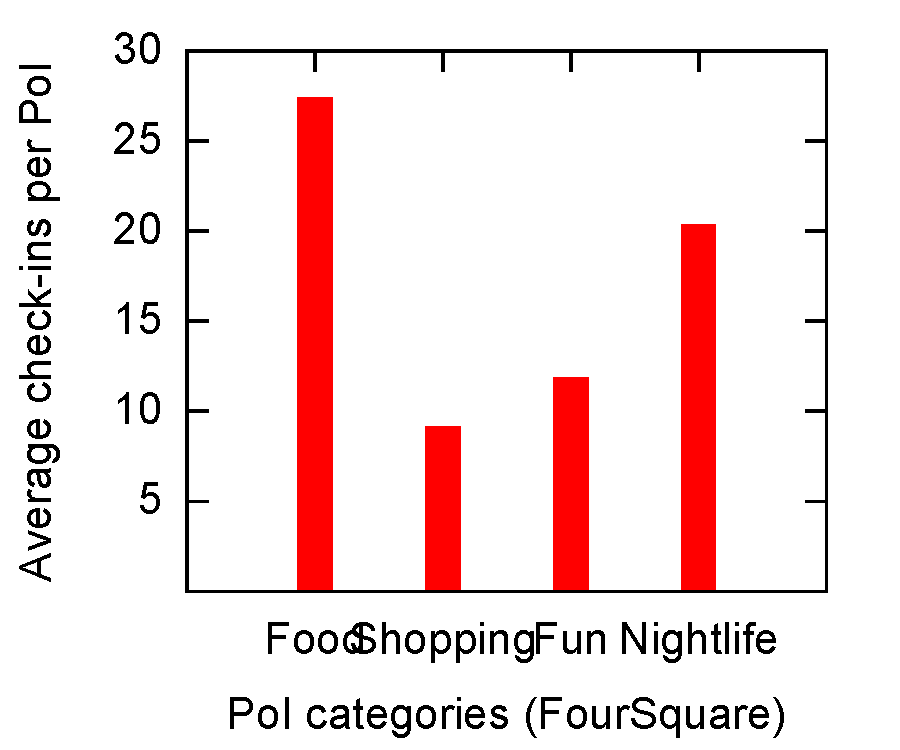
\includegraphics[scale=0.25]{E3-b.pdf}
        \end{subfigure}
         \caption{MSE of different PoI categories}\label{E3}
         \vspace{-2mm}
\end{figure}

We compare the Mean Square Error (MSE) of rating prediction results of the three schemes. We adjust the number of users and PoIs, respectively, and exam the performance trend of the schemes. For comparison, we also calculate the MSE of two baseline approaches: \textbf{Random} and \textbf{Average}. Random randomly generate a score in $[0,10]$ as user rating for each PoI, while Average uses the average rating of all the PoIs in the dataset as its prediction. The result is plotted in Figure~\ref{E12}. The proposed DNN prediction method demonstrate clear advantage over the other schemes for a moderate number of users. The performance of LR is also close to that of pure matrix factorization for larger number of users. The performance of DNN increases as the number of users increases. This implies a larger group of users overall have more reliable spatial-temporal features. In contrast, the performance of MF drops as the number of users/PoI increases. As the size of user-PoI rating matrix increases, it becomes more spares, making it harder for MF to generate accurate predicts. 

We also shows the MSE of the prediction result for PoIs in four different categories, namely ``Food", ``Shopping", ``Fun", and ``Nightlife". These PoI categories are provided by FourSquare. There appears to be a difference of prediction accuracy between PoI categories (Figure~\ref{E3}-a). For the proposed methods, the prediction result for ``Food" and ``Nightlife" shows a lower MSE comparing with that of ``Shopping" and ``Fun". A closer look at check-in data in different PoI category reveals that users reported less check-ins for ``Shopping" and ``Fun" PoIs comparing with that of `Food" and ``Nightlife" (Figure~\ref{E3}-b). Thus the relatively worse performance can be explained by the lack of data, which can affect the quality of extracted features.


\begin{figure}[htbp]%
        \centering
        \begin{subfigure}{0.25\textwidth}
               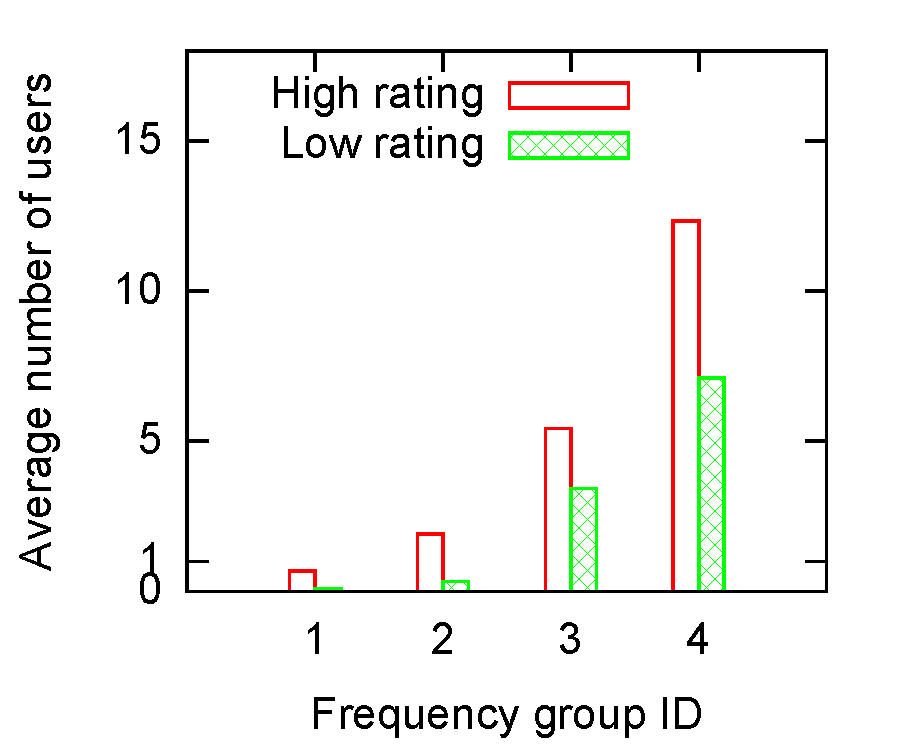
\includegraphics[scale=0.25]{E4-a.pdf}
        \end{subfigure}%
        ~ %add desired spacing between images, e. g. ~, \quad, \qquad, \hfill etc.
          %(or a blank line to force the subfigure onto a new line)
        \begin{subfigure}{0.25\textwidth}
                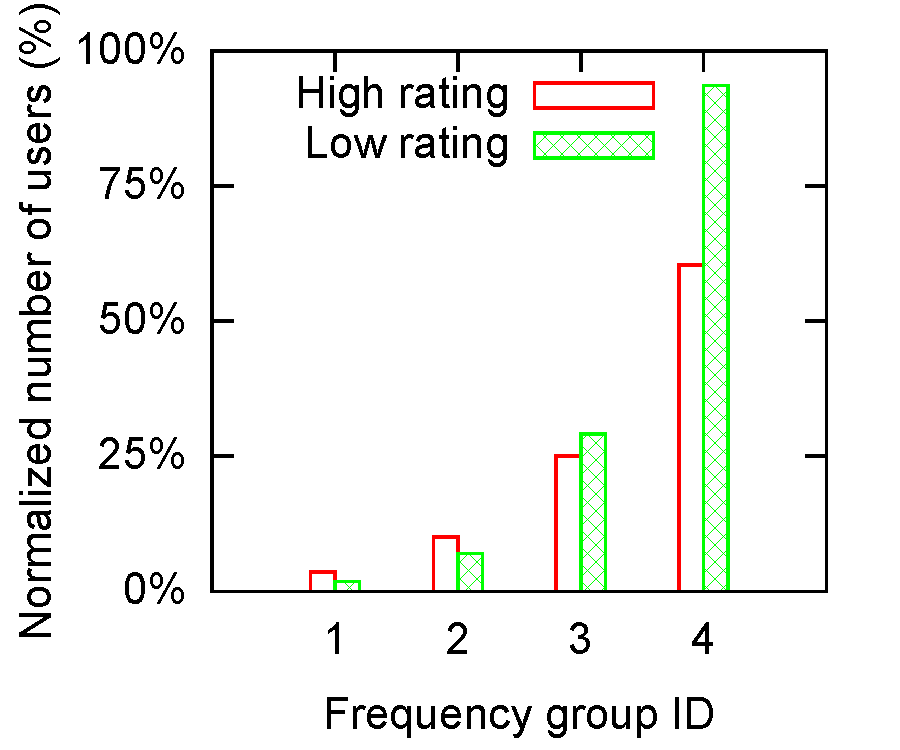
\includegraphics[scale=0.25]{E4-b.pdf}
        \end{subfigure}
         \caption{User frequency group distribution}\label{E4}
         \vspace{-2mm}
\end{figure}

Figure~\ref{E4} compares PoIs with different ratings in terms of the (normalized) average number of user in each frequency group, as showed in Table~\ref{frequencyGroups}. We define high rating PoI as a PoI with a overall score of 7.5 or higher out of 10. While a low rating PoI is one with an overall score of 2.5 or less. In general, highly rated PoIs have more visitors. Furthermore, we observe that a highly rated PoI attracts more frequent-visitors among all the visitors, comparing with PoIs with low ratings. These results support the assumptions we made in Section~\ref{sec:method}.
